\chapter{(Future) Methodology}
\label{cha:methodology}

\section{Data analysis}
\label{sec:method}

\begin{figure*}[h]
  \label{fig:flowchart}
  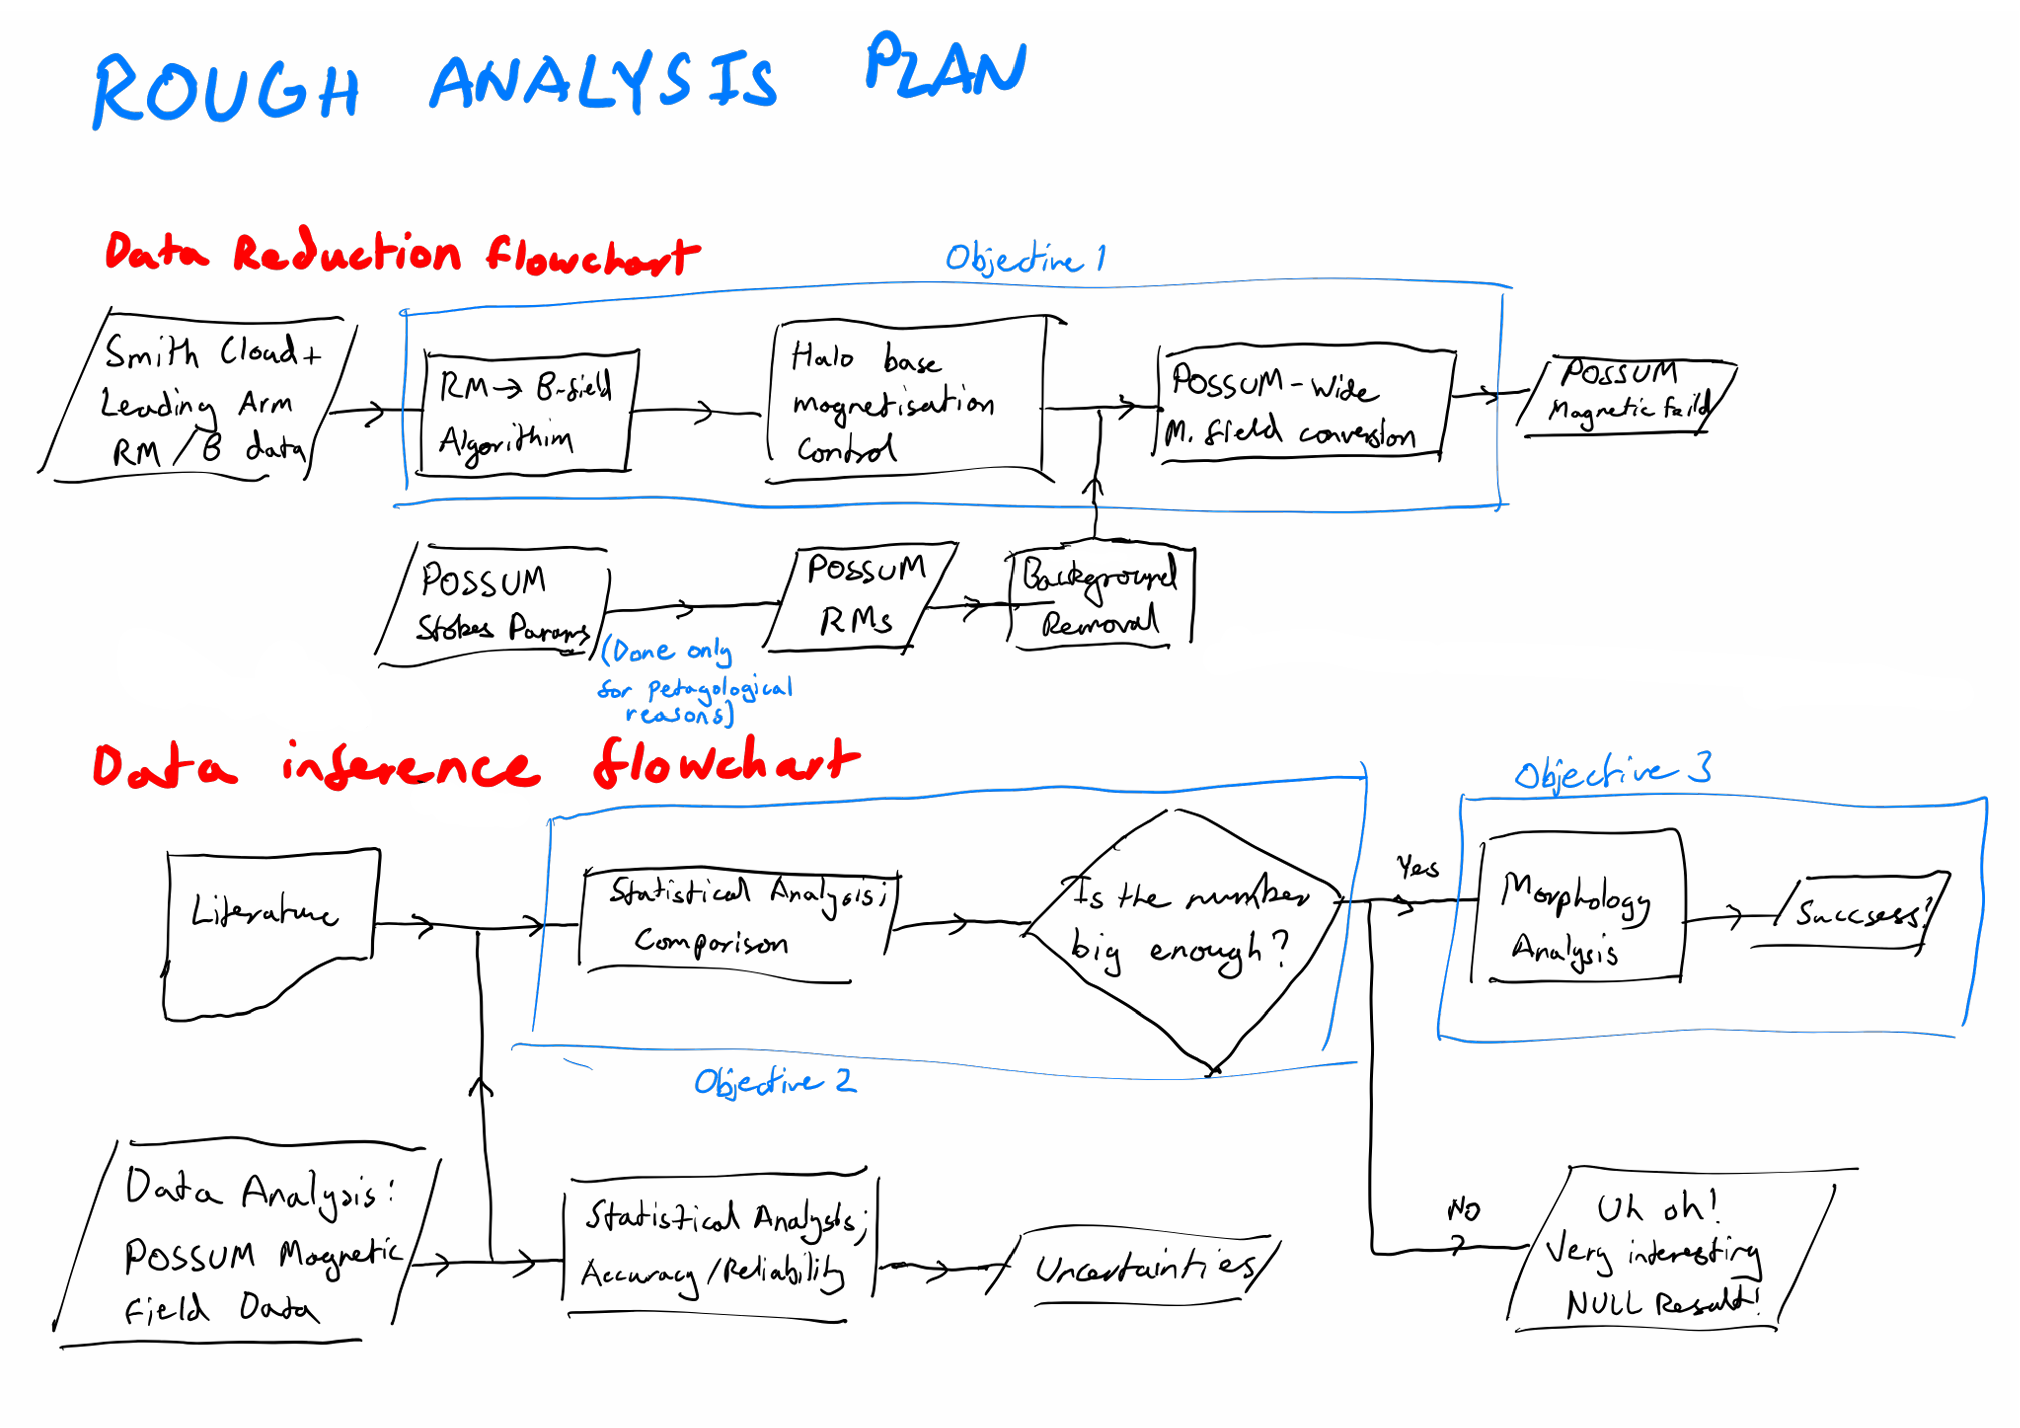
\includegraphics[width=\columnwidth]{figs/flowchart.png}
  \caption{A rough flowchart of the data analysis method. A neater version of this flowchart will appear in future iterations of the report as a visual representation of the methodology.}
\end{figure*}

Figure Figure~\ref{fig:flowchart} represents the rough outline of the pipeline of data analysis.

\section{Timeline of honours project}
\label{sec:timeline}

\begin{table*}[h]
  \centering
  \input table/timeline.tex
  \caption{A planned timeline of events.}
  \label{tab:timeline}
\end{table*}

Table~\ref{tab:timeline} displays a rough timeline of planned events over the year.


%%% Local Variables: 
%%% mode: latex
%%% TeX-master: "paper"
%%% End: 
